% Chapter 2

\chapter{Kingdomino} % Main chapter title

\label{Chapter2} % For referencing the chapter elsewhere, use \ref{Chapter1}

\section{Le jeu de société}
Le jeu Kingdomino est un jeu de société de prise de territoire utilisant des tuiles ou dominos de type de terrains différents. Le jeu se joue de 2 à 4 joueurs.\\
Le jeu est composé de :
\begin{itemize}
    \item 4 tuiles de départ neutre.
    \item 48 dominos avec une face paysage et une face numérotée.
    \item 8 rois de 4 couleurs différentes.
\end{itemize}

\begin{center}
  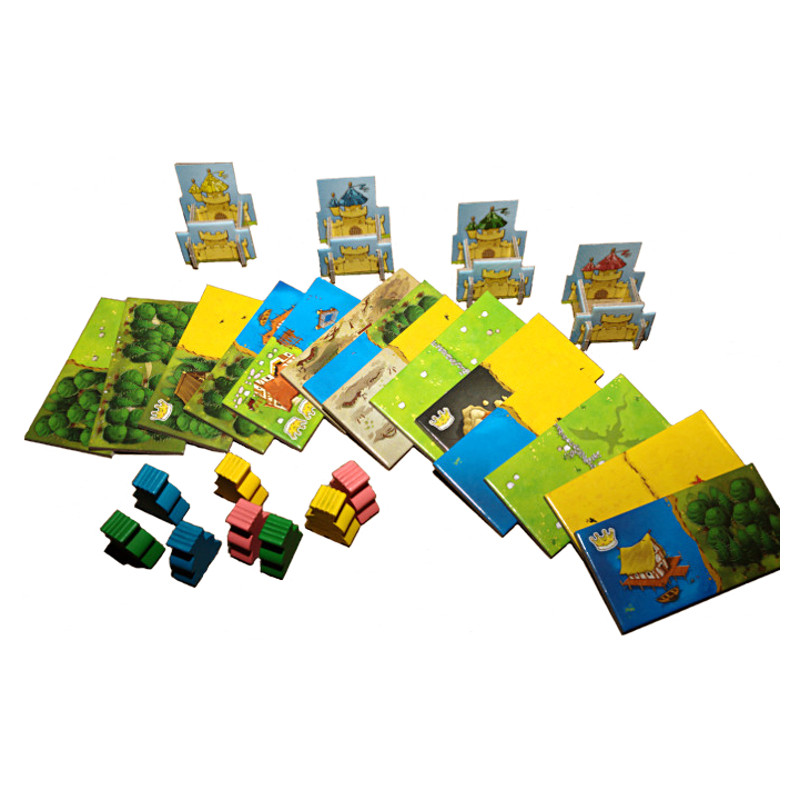
\includegraphics[scale=0.5]{Figures/jeuking}
  \caption{Kingdomino}
\end{center}

\subsection{But du jeu}
Le but du jeu est de connecter astucieusement vos dominos afin de construire le royaume de $5 \times 5$ cases le plus prestigieux et de marquer le plus de points possible.

%----------------------------------------------------------------------------------------
\newpage
\section{Les règles}

Les règles du jeu ne sont pas très compliquées mais soyez attentif :

\subsection{Le commencement}
Pour un jeu à 2 joueurs, on utilisera que 24 dominos.\\
Pour un jeu à 3 joueurs, on utilisera 36 dominos.\\
Et enfin, pour un jeu à 4 joueurs, on utilisera les 48 dominos.\\\\
L'ordre du premier tour de jeu est déterminé par de l'aléatoire, c'est un choix de notre part. Devant les joueurs il y a un pioche de tuiles, 4 par tour si le jeu se joue à 2 ou 4 joueurs sinon il y aura 3 tuiles devant les joueurs. Elles sont rangées par ordre croissant de numéro de tuile.\\
Chacun leur tour, les joueurs vont choisir quel domino ils veulent prendre parmis les 4  proposés (ou 3 si jeu à 3 joueurs) grâce a leur "roi", qu'ils vont placer sur le domino qu'ils convoitent, afin de compléter leur royaume et marquer un maximum de points.\\
\\
Exemple de pioche de tuile à 2 ou 4 joueurs :\\

\begin{center}
  
\includegraphics[scale=0.5]{Figures/tuiledistrib.png}
  \caption{tuile1}
\end{center}
\\ \\
Imaginons que le premier tour de jeu se passe comme cela :\\

\begin{center}
  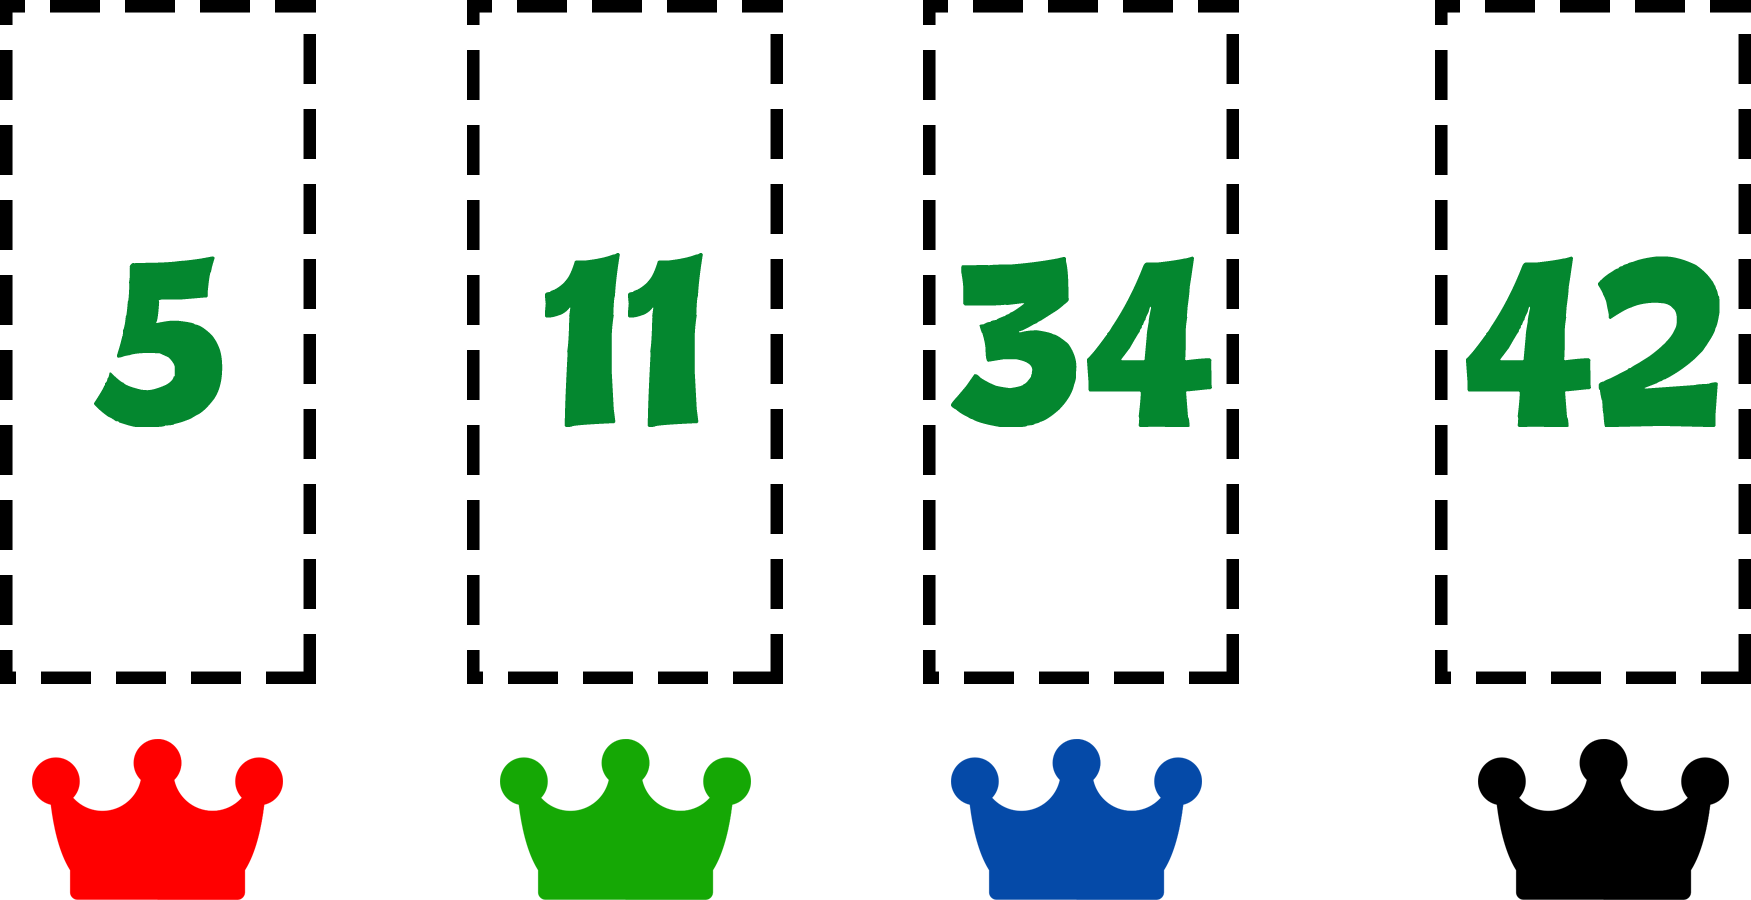
\includegraphics[scale=0.5]{Figures/tuileroi.png}
  \caption{tuile2}
\end{center}
\\ \\
Alors le roi  
\includegraphics[scale=0.3]{Figures/roirouge.png} sera le premier a jouer au tour suivant puisqu'il a choisi la tuile avec le numéro le plus petit entre les 4.
Logiquement, en deuxième c'est le roi 
\includegraphics[scale=0.3]{Figures/roivert.png} puis le roi 
\includegraphics[scale=0.3]{Figures/roibleu.png} et enfin le dernier le roi 
\includegraphics[scale=0.3]{Figures/roinoir.png}.\\
\\
Ainsi de suite jusqu'a la fin du jeu.

\newpage
\subsection{La connexion des tuiles}

Les joueurs doivent donc construire un royaume de $5 \times 5$ cases (un domino étant constitué de 2 cases).\\
Pour pouvoir poser son domino, le joueur doit :
\begin{itemize}
    \item Soit le connecter à son chateau de départ, qui est considéré comme une tuile joker (n'importe quel paysage peut être collé à ce domino).
\end{itemize}
\begin{center}
  
\includegraphics[scale=0.5]{Figures/tuilechateau.png}
  \caption{tuile3}
\end{center}
\begin{itemize}
    \item Soit le connecter à un autre domino en faisant correspondre au minimum 1 paysage (horizontalement ou verticalement uniquement).
\end{itemize}
\begin{center}
  
\includegraphics[scale=0.5]{Figures/2tuiles.png}
  \caption{tuile4}
\end{center}
\\
Dans le cas où il est impossible de venir ajouter un domino à son royaume en respectant les règles ci-dessus, le domino est défaussé et ne rapportera aucun point.\\\\
Tous les dominos doivent tenir dans un espace de $ 5 \times 5$ cases.\\\\
En cas de mauvaise anticipation, un à plusieurs dominos pourraient ne plus être exploitables et seront défaussés. Ils ne rapporteront alors aucun point.

\newpage
\subsection{Le fin du jeu}

Lorsque les derniers dominos sont placés en ligne au milieu de la table, les joueurs jouent un dernier tour normalement.\\
Chaque joueur devrait alors avoir devant lui un royaume de $5 \times 5$ cases. (Certains royaumes peuvent être incomplets si le joueur a été obligé de défausser des dominos.)\\
Chaque joueur va calculer les points de prestige de son royaume de la façon suivante :
\begin{itemize}
    \item Un royaume est constitué de différents \textbf{DOMAINES} (groupe de cases connectées horizontalement ou verticalement du même type de terrain).
    \item Chaque domaine rapporte autant de points de prestige que son \textbf{NOMBRE DE CASES} multiplié par le \textbf{NOMBRE DE COURONNES} présentes sur le domaine.
    \item Il peut y avoir plusieurs domaine du même type de terrain dans un même royaume.
    \item Un domaine sans couronne ne rapport aucun point.
    \item Chaque joueur additionne les points rapportés par chacun de ses domaines, le résultat de cette addition lui donne son score final.
    \item Le joueur qui a le plus haut score gagne la partie.
    \item En cas d'égalité, le joueur qui a construit le domaine le plus étendus, remporte la partie. Si cela ne suffit pas, c'est celui qui a le plus de couronne et si cela ne suffit toujours pas alors ils ont gagné tous les deux.
\end{itemize}

\begin{center}
  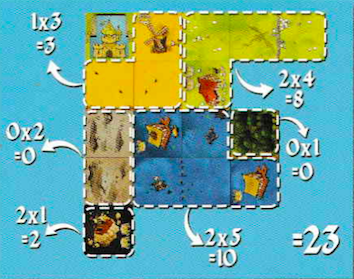
\includegraphics[scale=0.5]{Figures/exFindeJeu.png}
  \caption{FinDeJeu}
\end{center}

\subsection{Règles additionnelles et optionnelles}

Il existe des règles additionnelles et optionnelles pour des modes de jeu différents mais nous sommes rester dans les limites des règles du jeu classique.

%----------------------------------------------------------------------------------------